Applying the usual model architecture with PCC loss too train the model to predict fluorescence signal from DIC imaging for Golgi did not bring a good results. Model seems to converge (see Figure \ref{fig:golgi-no-reg-pcc}), however there is no learning happening.
\begin{figure}[H]
	\begin{center}
		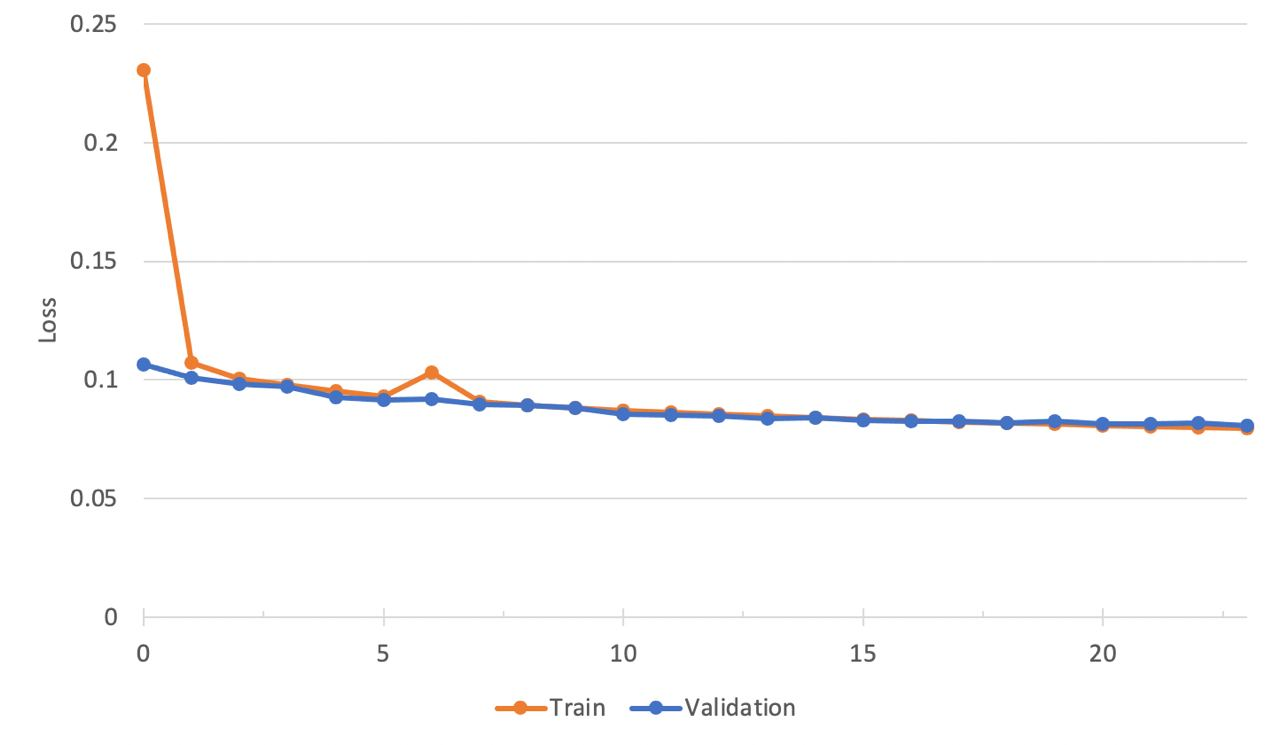
\includegraphics[width=0.5\linewidth]{bilder/golgi/pcc-no-reg.jpg}
		\caption{Straightforward training doesn't work}\label{fig:golgi-no-reg-pcc}
	\end{center}
\end{figure}

This was also depicted in visual predictions where the predicted fluroescence mostly contains dark pixels only (see Figure \ref{fig:golgi-no-reg-pcc-predictions}). Altough it seems that some pattern is hidden behind the dark pixels, visualizing it simply shows that the model picks up on the cell outline itself and does not give any useful information on the location of Golgi. One can see this by normalizing the predicted dark image to the range $[0,1]$ (Figure \ref{fig:golgi-no-reg-pcc-predictions}).
\begin{figure}[htb]
	\begin{center}
		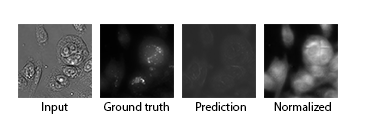
\includegraphics[width=0.8\linewidth]{bilder/golgi/too-dark.png}
		\caption{Training on original data}\label{fig:golgi-no-reg-pcc-predictions}
	\end{center}
\end{figure}

While in Figure \ref{fig:golgi-no-reg-pcc-predictions} only the results of predictions for one crop are presented, it would be interesting to see how the image with combines crops would look like. This is presented in Figure \ref{fig:golgi-no-reg-pcc-predictions-full}. One can notice an interesting pattern there: essentially the model is predicting some signal across the whole cell with a brighter regions in some of them. Yet these regions do not have a correct location wrt to Golgi. Also it is important to keep in mind, that the image of the right in this Figure is a normalized one and a true image is almost fully black. 
\begin{figure}[htb]
	\begin{center}
		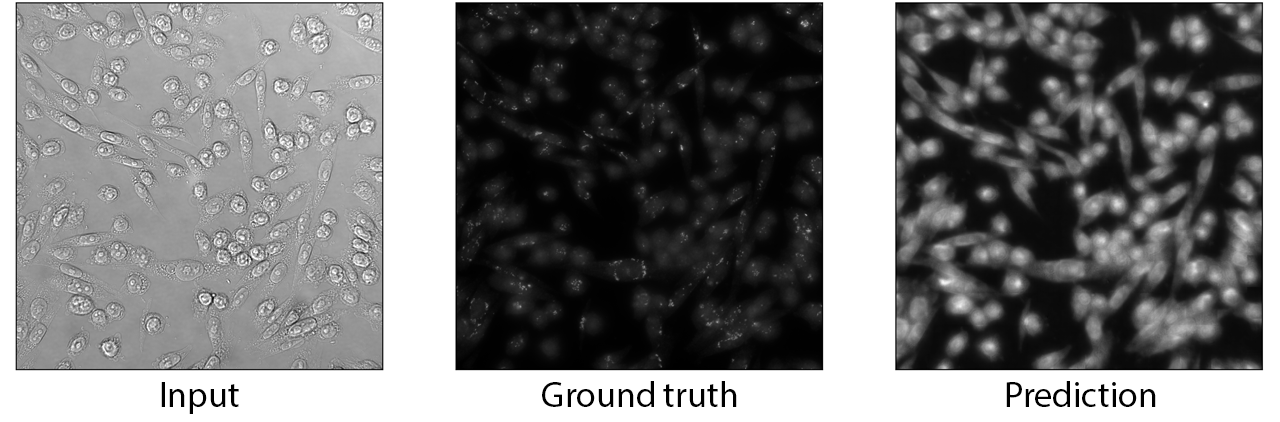
\includegraphics[width=0.8\linewidth]{bilder/golgi/full-img.png}
		\caption{Full size predictions}\label{fig:golgi-no-reg-pcc-predictions-full}
	\end{center}
\end{figure}

This experiment brought a hypothesis that the background removal algorithm might have reduces the signal-to-noise ratio and remove some important fluroescence signal along the way. Therefore an alternative approach of a background removal had been tried, where only enhancing via clipping described above has been applied directly on fluprescence imaging (without using a rolling ball algorithm). This produces images that still have much more non-specific fluorescence background (see Figure \ref{fig:golgi-enhanced-predictions} (second image)), yet this preprocessing alternates the initial image to a much lower extent. 

\begin{figure}[htb]
	\begin{center}
		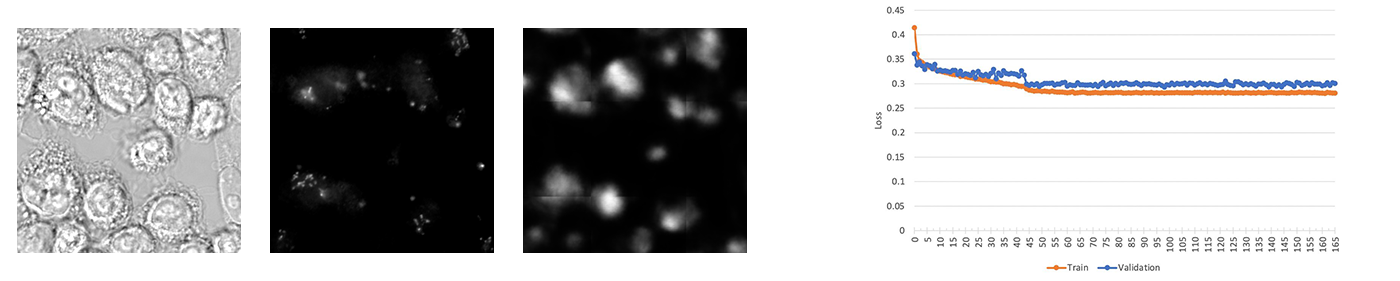
\includegraphics[width=\linewidth]{bilder/golgi/enhanced-crop.png}
		\caption{Training on the enhanced data}\label{fig:golgi-enhanced-predictions}
	\end{center}
\end{figure}
In this case predictions are not completely black anymore, however their quality is still very low. Images used in these training experiments were effectively coming from different staining procedures, using different antibodies, fixation process and microscopy settings. This brought up an idea to train the model on few selective datasets only that were created with the first staining approach only. The preprocessing was chosen as in the previous example --- with the use of enhancement and without rolling ball algorithm as it has shown the best results.

\begin{figure}[htb]
	\begin{center}
		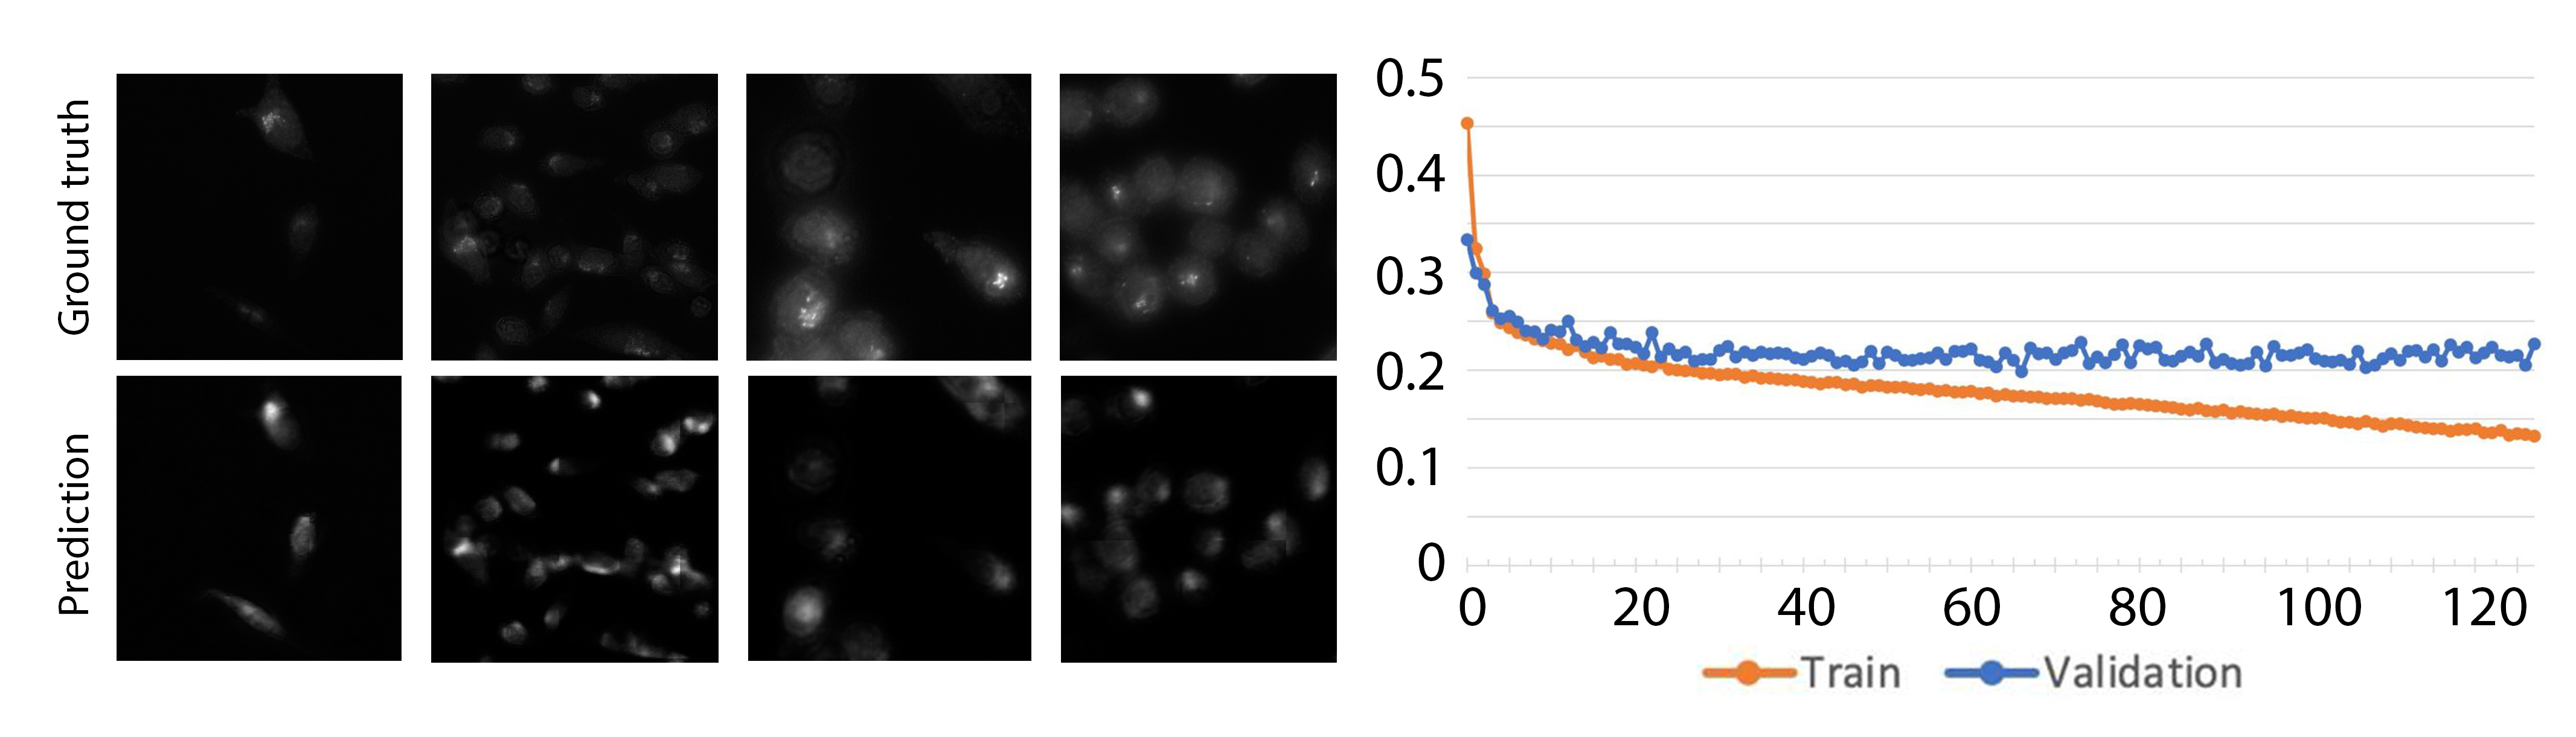
\includegraphics[width=\linewidth]{bilder/golgi/12-13/12-13.png}
		\caption{Small subset of the best staining}\label{fig:12-13}
	\end{center}
\end{figure}

The predictions from this experiment you can find in Figure \ref{fig:12-13}. Due to the stricter filtering and the use of much less data there were much smaller crops which were used for training. In this case only $4251$ crops were used for training and $406$ for validation purposes, which directly led to overfitting after $70$ epochs. However, the predictions did improve visually as well as the loss dropped to $0.19$. Nevertheless the losses from these two experiments should not be compared directly as they were evaluated on two different validation sets. The improvement of the results indicated the careful choice of data samples taken from the same staining approach with the same settings, that does not require a severe preprocessing and already has a high signal-to-noise ratio might help the predictions significantly. There is a potential here for a better regularization of the model trained on the small subset of data. Yet it is clear that the acquisition of a better fluorescence staining is much more crucial here.